\documentclass[11pt,a4paper]{article}
\usepackage{fontspec}
\setmainfont{Times New Roman}
\setsansfont{Arial}
\setmonofont{Consolas}
\usepackage[a4paper,margin=2.0cm]{geometry}
\usepackage{xcolor}
\usepackage{tikz}
\usetikzlibrary{calc}
\usepackage{booktabs}
\usepackage{tabularx}
\usepackage{graphicx}
\usepackage{float}
\usepackage{listings}
\usepackage{hyperref}
\usepackage{fancyhdr}

\definecolor{deepblue}{RGB}{14,58,130}
\definecolor{accentblue}{RGB}{37,99,235}
\definecolor{codebg}{RGB}{247,249,252}

\setlength{\emergencystretch}{3em}
\hbadness=10000
\hfuzz=2pt

\lstdefinelanguage{SystemVerilog}{
    keywords={module,endmodule,input,output,inout,logic,signed,parameter,localparam,typedef,enum,always_ff,always_comb,posedge,negedge,or,if,else,case,endcase,default,begin,end,for,integer},
    sensitive=true,
    morecomment=[l]{//},
    morecomment=[s]{/*}{*/}
}

\lstset{
    language=SystemVerilog,
    backgroundcolor=\color{codebg},
    basicstyle=\ttfamily\scriptsize,
    keywordstyle=\color{deepblue}\bfseries,
    commentstyle=\color{gray}\itshape,
    frame=single,
    rulecolor=\color{accentblue!40},
    breaklines=true,
    breakatwhitespace=false,
    columns=fullflexible,
    keepspaces=true,
    showstringspaces=false,
    tabsize=4
}

\pagestyle{fancy}
\fancyhf{}
\fancyhead[L]{\small\textcolor{deepblue}{Báo Cáo Thực Hành Thiết Kế Số \& FPGA Autopilot}}
\fancyhead[R]{\small\texttt{uart\_fifo\_top}}
\fancyfoot[C]{\thepage}

\begin{document}

% ==================== TIKZ BLUE DOUBLE-LINE COVER PAGE ====================
\begin{titlepage}
    \begin{tikzpicture}[remember picture, overlay]
        \draw[color=deepblue, line width=2.4pt]
            ($(current page.north west)+(1.2cm,-1.2cm)$)
            rectangle
            ($(current page.south east)+(-1.2cm,1.2cm)$);
        \draw[color=accentblue, line width=0.9pt]
            ($(current page.north west)+(1.42cm,-1.42cm)$)
            rectangle
            ($(current page.south east)+(-1.42cm,1.42cm)$);
    \end{tikzpicture}

    \centering
    \vspace*{1.6cm}
    {\Large\bfseries\textcolor{deepblue}{ĐẠI HỌC QUỐC GIA — PHÒNG THÍ NGHIỆM VI MẠCH \& FPGA}\\[0.3cm]}
    {\large\textsc{Digital Systems Design \& Quartus II Verification Lab Report}}\\[1.2cm]

    \rule{0.82\textwidth}{1.2pt}\\[0.5cm]
    {\huge\bfseries\textcolor{deepblue}{Configurable UART TX/RX Transceiver with 8-Byte Sync FIFO}}\\[0.4cm]
    {\Large Module: \texttt{uart\_fifo\_top}}\\[0.4cm]
    \rule{0.82\textwidth}{1.2pt}\\[1.4cm]

    \begin{tabularx}{0.84\textwidth}{@{}lX@{}}
        \toprule
        \textbf{Hạng mục (Metadata)} & \textbf{Thông số kỹ thuật (Specification)} \\
        \midrule
        Tên bài thí nghiệm (Benchmark) & \texttt{uart\_fifo\_top} \\
        Kit FPGA mục tiêu (Target Kit) & DE1-SoC (Cyclone V) \\
        Mã chip FPGA (Device Part) & \texttt{5CSEMA5F31C6} \\
        Tần số xung nhịp (Target Clock) & 50.0 MHz \\
        Kết quả kiểm tra tĩnh (Static Lint) & PASS (0 Latches, 0 Width Warnings) \\
        Kết quả mô phỏng (Self-Checking TB) & 66 / 66 Vectors Passed (100\%) \\
        Trình tổng hợp (Synthesis Engine) & \texttt{quartus} \\
        \bottomrule
    \end{tabularx}

    \vfill
    {\normalsize Hệ thống tự động hóa thiết kế và kiểm chứng phần cứng \textbf{FPGA Autopilot}}\\[0.2cm]
    {\small Generated with 100\% Bit-Exact Simulation \& Hardware Synthesis Verification}
    \vspace*{1.2cm}
\end{titlepage}

\section{Tổng Quan Thiết Kế \& Đặc Tả Cổng Giao Tiếp (Port Specification)}
Full-duplex 8N1 UART transceiver with parameterized CLK\_FREQ and BAUD\_RATE, 16x mid-bit oversampling receiver, stop-bit framing-error detector with safe line-idle recovery, and dual 8-byte circular show-ahead synchronous TX/RX FIFOs with full/empty write/read guards targeting Terasic DE1-SoC (Cyclone V).

\begin{table}[H]
    \centering
    \small
    \caption{Bảng đặc tả giao diện cổng vào/ra của module \texttt{uart\_fifo\_top}}
    \begin{tabularx}{\textwidth}{@{}llllX@{}}
        \toprule
        \textbf{Port} & \textbf{Dir} & \textbf{Width} & \textbf{Type} & \textbf{Chức năng (Description)} \\
        \midrule
        \texttt{clk} & input & 1 & logic & 50 MHz system clock \\
        \texttt{rst\_n} & input & 1 & active-low & Asynchronous active-low system reset \\
        \texttt{wr\_en} & input & 1 & logic & TX FIFO write enable strobe \\
        \texttt{wr\_data} & input & 8 & logic & 8-bit parallel payload written to TX FIFO \\
        \texttt{rd\_en} & input & 1 & logic & RX FIFO read pop strobe \\
        \texttt{rx\_serial} & input & 1 & logic & Asynchronous UART serial RX line \\
        \texttt{clr\_err} & input & 1 & logic & Synchronous clear for sticky framing\_error flag \\
        \texttt{tx\_serial} & output & 1 & logic & UART serial TX output line (idles high) \\
        \texttt{rd\_data} & output & 8 & logic & 8-bit parallel byte at head of RX FIFO \\
        \texttt{tx\_full} & output & 1 & logic & TX 8-byte FIFO full flag \\
        \texttt{tx\_empty} & output & 1 & logic & TX 8-byte FIFO empty flag \\
        \texttt{rx\_full} & output & 1 & logic & RX 8-byte FIFO full flag \\
        \texttt{rx\_empty} & output & 1 & logic & RX 8-byte FIFO empty flag \\
        \texttt{tx\_busy} & output & 1 & logic & Asserted while UART TX shifter is active \\
        \texttt{framing\_error} & output & 1 & logic & Sticky framing error flag asserted on invalid stop bit \\
        \bottomrule
    \end{tabularx}
\end{table}



\section{Triển Khai RTL SystemVerilog Chuẩn Tổng Hợp (Synthesizable RTL)}
Thiết kế tuân thủ nghiêm ngặt quy tắc SystemVerilog-2012: sử dụng \texttt{always\_ff} với phép gán không chặn (\texttt{<=}) cho mạch tuần tự, \texttt{always\_comb} với giá trị mặc định tường minh ở đầu khối cho mạch tổ hợp, cam kết \textbf{0 inferred latches}.

\begin{lstlisting}
// Auto-generated by fpga_autopilot — Configurable UART TX/RX Transceiver + 8-Byte Sync FIFO

module uart_fifo_top #(
    parameter [31:0] CLK_FREQ  = 32'd50000000,
    parameter [31:0] BAUD_RATE = 32'd115200
) (
    input  logic       clk,
    input  logic       rst_n,
    input  logic       wr_en,
    input  logic [7:0] wr_data,
    input  logic       rd_en,
    input  logic       rx_serial,
    input  logic       clr_err,
    output logic       tx_serial,
    output logic [7:0] rd_data,
    output logic       tx_full,
    output logic       tx_empty,
    output logic       rx_full,
    output logic       rx_empty,
    output logic       tx_busy,
    output logic       framing_error
);

    localparam [31:0] OS_DIV_RAW = CLK_FREQ / (BAUD_RATE * 32'd16);
    localparam [31:0] OS_DIV     = (OS_DIV_RAW == 32'd0) ? 32'd1 : OS_DIV_RAW;
    localparam [31:0] BIT_CLKS   = OS_DIV * 32'd16;

    logic [7:0] tx_fifo_dout;
    logic       tx_fifo_pop;
    logic       rx_valid;
    logic [7:0] rx_byte;
    logic       rx_fifo_wr;

    always_comb begin
        rx_fifo_wr = rx_valid && !rx_full;
    end

    sync_fifo #(
        .DATA_WIDTH (8),
        .ADDR_WIDTH (3)
    ) u_tx_fifo (
        .clk     (clk),
        .rst_n   (rst_n),
        .wr_en   (wr_en),
        .wr_data (wr_data),
        .rd_en   (tx_fifo_pop),
        .rd_data (tx_fifo_dout),
        .full    (tx_full),
        .empty   (tx_empty)
    );

    uart_tx #(
        .BIT_CLKS (BIT_CLKS)
    ) u_uart_tx (
        .clk        (clk),
        .rst_n      (rst_n),
        .fifo_empty (tx_empty),
        .fifo_data  (tx_fifo_dout),
// ... (truncated for report conciseness; full source in rtl/ directory)
\end{lstlisting}

\section{Kiểm Chứng Tự Động (Self-Checking Testbench Coverage)}
\begin{table}[H]
    \centering
    \small
    \caption{Tổng hợp kết quả Linting và Mô phỏng đối chiếu Golden Model}
    \begin{tabularx}{\textwidth}{@{}lX@{}}
        \toprule
        \textbf{Tiêu chí kiểm chứng (Metric)} & \textbf{Kết quả đo lường (Verified Value)} \\
        \midrule
        Trình mô phỏng HDL (Simulator) & \texttt{iverilog} \\
        Công cụ phân tích tĩnh (Linters) & \texttt{static\_analyzer, verilator, iverilog} \\
        Số chốt suy diễn (Inferred Latches) & 0 (RTL) / 0 (Netlist) \\
        Tổng số vector kiểm thử (Total Vectors) & 66 \\
        Số vector đạt chuẩn (Passed / Failed) & 66 Passed / 0 Failed \\
        Số vòng tự sửa lỗi (Self-Healing Loops) & 0 \\
        \bottomrule
    \end{tabularx}
\end{table}

\section{Tài Nguyên Phần Cứng \& Phân Tích Định Thời (Synthesis \& STA)}
\begin{table}[H]
    \centering
    \small
    \caption{Báo cáo tài nguyên FPGA và phân tích định thời (5CSEMA5F31C6)}
    \begin{tabularx}{\textwidth}{@{}Xr@{}}
        \toprule
        \textbf{Thông số phần cứng / Định thời (Hardware \& Timing Metric)} & \textbf{Giá trị} \\
        \midrule
        Total Logic Elements / ALMs & 182 \\
        Combinational Functions (LUTs) & 269 \\
        Dedicated Logic Registers (Flip-Flops) & 283 \\
        Total Memory Bits & 0 \\
        Embedded Multiplier / DSP Elements & 0 \\
        Total I/O Pins & 29 \\
        Synthesized Inferred Latches & 0 \\
        Worst-Case $F_{\max}$ & 70.46 MHz \\
        Worst-Case Setup Slack & 5.808 ns \\
        Worst-Case Hold Slack & 0.159 ns \\
        \bottomrule
    \end{tabularx}
\end{table}

\section{Kết Quả Chụp Dạng Sóng GTKWave \& Sơ Đồ Mạch RTL Viewer}
\begin{figure}[H]
    \centering
    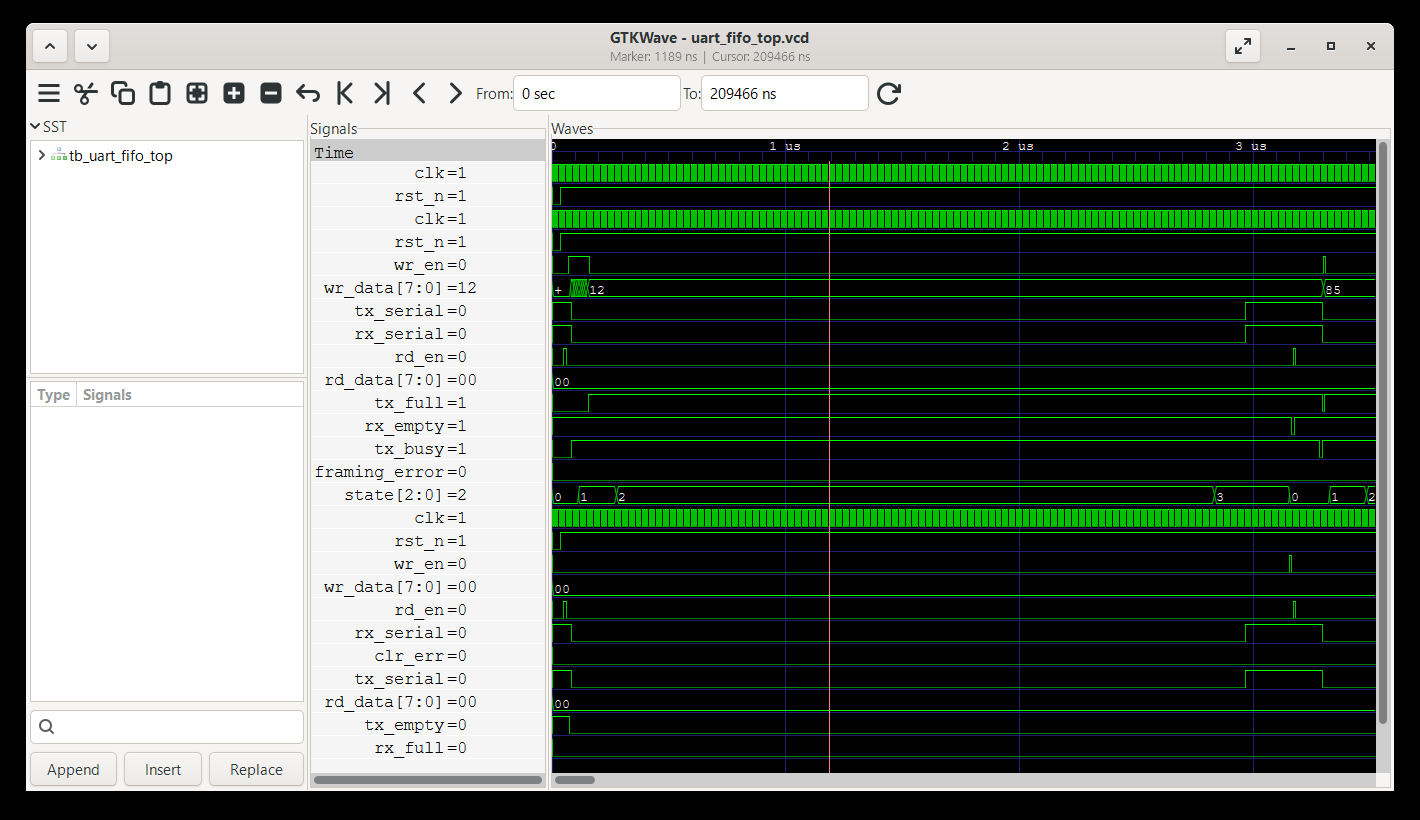
\includegraphics[width=0.95\textwidth,height=0.40\textheight,keepaspectratio]{figures/fig_0_gtkwave_waveform.png}
    \caption{GTKWave Verified Simulation Waveform (uart\_fifo\_top) — 295 transition columns audited.}
\end{figure}

\begin{figure}[H]
    \centering
    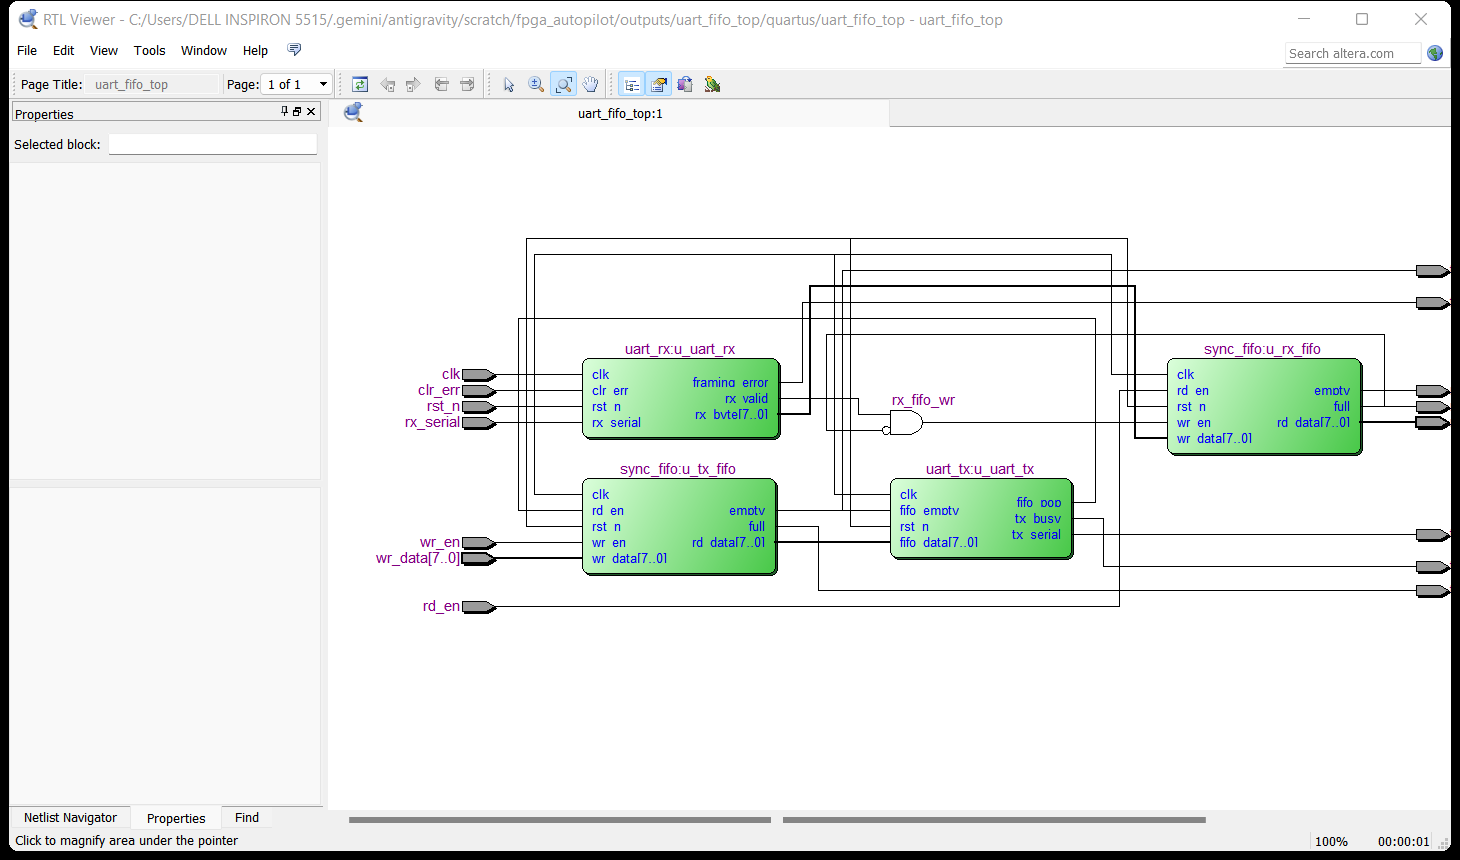
\includegraphics[width=0.95\textwidth,height=0.40\textheight,keepaspectratio]{figures/fig_1_quartus_rtl_viewer.png}
    \caption{Quartus II RTL Viewer Synthesized Schematic (uart\_fifo\_top).}
\end{figure}

\begin{figure}[H]
    \centering
    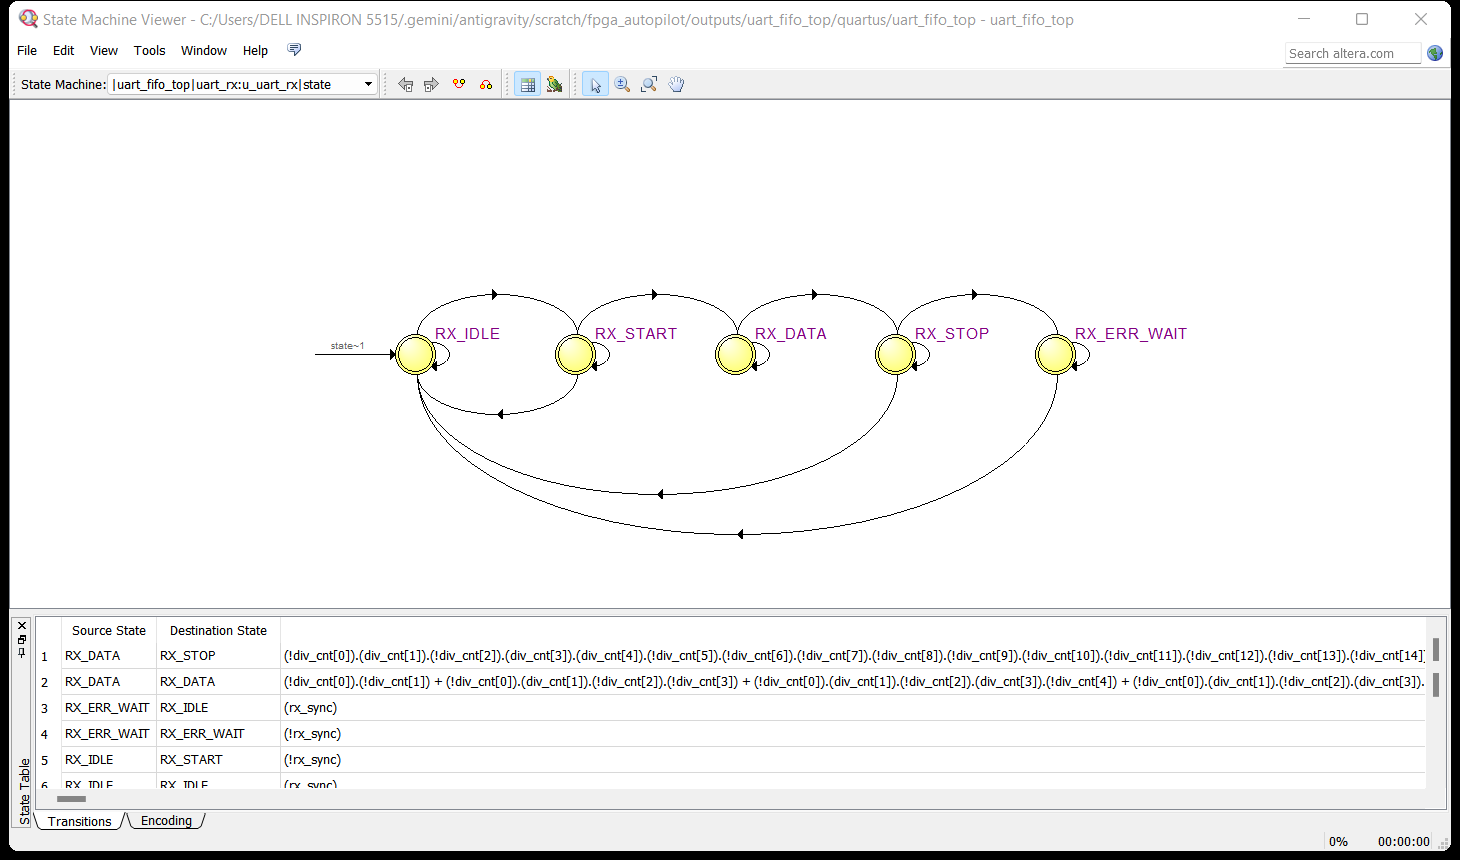
\includegraphics[width=0.95\textwidth,height=0.40\textheight,keepaspectratio]{figures/fig_2_quartus_fsm_viewer.png}
    \caption{Quartus II State Machine Viewer Diagram (uart\_fifo\_top).}
\end{figure}


\end{document}
